\documentclass[preprint,12pt,authoryear]{elsarticle}

\usepackage{amsmath}
\usepackage{booktabs}
\usepackage{graphicx}
\usepackage{hyperref}
\usepackage{siunitx}
\usepackage{subcaption}
\usepackage{threeparttable}

\sisetup{detect-all=true}
\emergencystretch=2em
\journal{Spectrochimica Acta Part B: Atomic Spectroscopy}
\bibliographystyle{elsarticle-harv}

\begin{document}

\begin{frontmatter}

\title{Physics-constrained element identification for low-resolution calibration-free LIBS: a benchmark on mineral spectra}

\author[inst1]{Brian Squires}
\affiliation[inst1]{organization={CF-LIBS Project}}

\begin{abstract}
Blind element identification remains a limiting step for calibration-free laser-induced breakdown spectroscopy (CF-LIBS), especially for compact instruments whose resolving powers are too low to support unambiguous line assignment. We evaluate five element-identification pathways on 74 low-resolution LIBS spectra from a mineral and pure-element benchmark: ALIAS peak matching, full-spectrum non-negative least squares (NNLS), a two-stage NNLS+ALIAS hybrid, Voigt deconvolution followed by ALIAS, and forward-model coefficient thresholding. The spectra span 200--900 nm at effective resolving powers of approximately 300--1100 and are scored as 22-element multi-label detections using micro-averaged precision, recall, F$_1$, false-positive rate, and exact-match rate. The hybrid method in intersection mode gives the best overall result, with precision 0.604, recall 0.713, F$_1$ 0.654, false-positive rate 0.053, and 16 exact matches among 74 spectra. This represents a 16.8\% relative F$_1$ improvement over the best ALIAS baseline. Full-spectrum NNLS reaches high recall (0.940) but low precision (0.293), whereas ALIAS provides moderate precision (0.505) and recall (0.629). The hybrid improves performance by using NNLS as a global, physically constrained candidate screen and ALIAS as a line-level confirmation step. Per-element analysis shows reliable high-precision behavior for Si, Al, Fe, Li, Co, and Ni, but Mn and Na remain dominant false-positive sources. The results indicate that low-resolution blind LIBS element identification is not solved by peak matching or full-spectrum fitting alone. A conservative two-stage architecture provides the strongest result among the evaluated pathways, while specimen-specific chemical validation, uncertainty estimates, higher-resolution comparisons, and calibration-robust benchmarks are needed before the method can support quantitative CF-LIBS in unknown field samples.
\end{abstract}

\begin{keyword}
laser-induced breakdown spectroscopy \sep calibration-free LIBS \sep element identification \sep NNLS \sep spectral unmixing \sep mineral spectroscopy \sep low-resolution spectrometry
\end{keyword}

\end{frontmatter}

\begin{figure}[t]
  \centering
  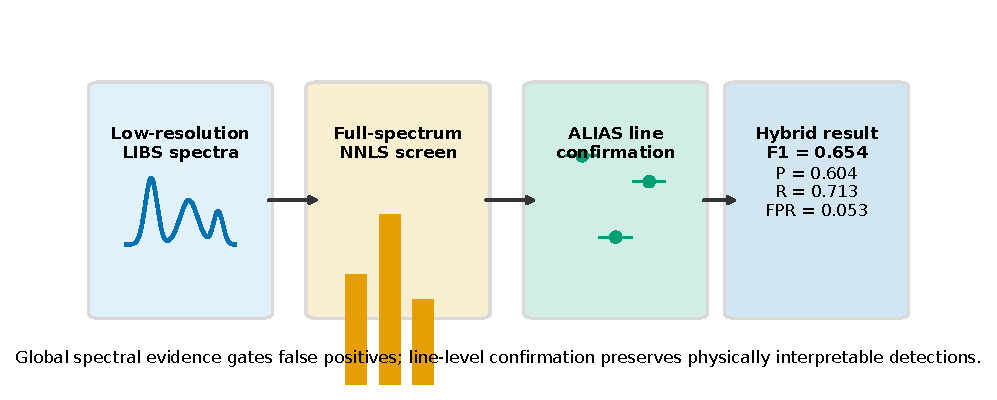
\includegraphics[width=0.92\linewidth]{figures/graphical_abstract.pdf}
  \caption{Graphical abstract. Low-resolution LIBS spectra are screened by full-spectrum NNLS, confirmed by ALIAS line evidence, and scored as multi-label element detections. The best hybrid operating point improves precision relative to NNLS and recall relative to ALIAS while preserving a low false-positive rate.}
  \label{fig:graphical}
\end{figure}

\section{Introduction}

Laser-induced breakdown spectroscopy (LIBS) uses a focused laser pulse to form a transient plasma and records atomic and ionic emission from the ablated material. The technique is attractive for geological, industrial, environmental, and planetary measurements because it is rapid, minimally preparative, and compatible with remote operation. Calibration-free LIBS (CF-LIBS) seeks to convert spectra into elemental abundances without matrix-matched standards by combining Saha--Boltzmann population models, plasma diagnostics, and a closure equation \citep{Ciucci1999,Tognoni2010}. This ambition is especially important when representative calibration standards are unavailable, as in planetary exploration or field measurements of heterogeneous materials. However, CF-LIBS is only as reliable as the element list supplied to the quantitative solver. If an absent element is included, its lines and continuum contributions can distort temperature estimates, partition the closure equation incorrectly, and perturb the inferred concentrations of all other species. If a present element is omitted, its emission is forced into residuals or spuriously assigned to other species.

Element identification is comparatively straightforward when lines are isolated and instrumental resolution is high. It becomes much harder in compact or field-deployed spectrometers whose resolving powers are often below 1000. Over a broad 200--900 nm band, such instruments compress thousands of catalogued atomic transitions into a few hundred independent resolution elements. Apparent peaks are therefore frequently blend envelopes rather than individual transitions. Peak-matching algorithms can still be useful, but chance coincidences become common, especially for line-rich elements, and low-abundance or strongly blended elements may fall below detection thresholds. This is the same information bottleneck that has motivated multivariate, submodel, and calibration-library approaches in operational Mars LIBS pipelines \citep{Wiens2012,Maurice2012,Wiens2013,Clegg2009,Anderson2017}. It has also motivated community benchmark datasets for supervised LIBS classification \citep{Kepez2020}. Those resources are powerful when large, representative training libraries exist, but a calibration-free workflow still needs reliable element decisions in more open-ended compositional settings.

The present work asks a deliberately narrow question: among physics-based and semi-physics-based methods available in the current CF-LIBS codebase, which pathway provides the strongest baseline for blind element identification at low resolving power? The question is distinct from mineral classification and from quantitative abundance prediction. A mineral classifier can correctly name a sample while failing to report all elements, and a regression model can predict a fixed set of oxides without solving the open-world decision of which elements should enter a CF-LIBS calculation. We therefore frame the task as multi-label element detection and score each method using precision, recall, F$_1$, false-positive rate, and exact-match count.

We compare five pathways. The first is ALIAS-style peak matching, which represents line-evidence confirmation against an atomic database \citep{Labutin2013,Amato2010}. The second is full-spectrum NNLS decomposition, in which the observed spectrum is fit as a non-negative combination of Saha--Boltzmann basis spectra. The third is a two-stage hybrid that uses NNLS for high-recall candidate screening and ALIAS for line-level confirmation. The fourth tests whether Voigt deconvolution can rescue peak matching by sharpening blended features. The fifth applies a concentration-like threshold to forward-model coefficients. The scientific contribution is not a claim that low-resolution identification is solved. It is a quantitative and reproducible benchmark showing where physically constrained screening helps, where it fails, and which validity limits must be addressed before such a pipeline can be trusted for field CF-LIBS.

\section{Methods}

\subsection{Benchmark spectra and reference labels}

The benchmark consists of 74 LIBS spectra: 13 pure-element targets and 61 mineral spectra compiled from the public Aalto LASOLIBS dataset pages \citep{AaltoDatasets2025}. The source page describes downloadable LIBS datasets in NetCDF or MATLAB/HDF5-compliant formats and identifies pure-element and mineral datasets, with the mineral collection described as mostly from Aalto University collections. The page is explicitly marked as a draft research webpage, so it is treated here as a public data source rather than as a peer-reviewed dataset publication. The spectra cover approximately 200--900 nm, and effective resolving power estimated from isolated peak widths spans approximately 300--1100, with most spectra in the low-resolution regime where peak matching is expected to be difficult. The evaluated element universe contains 22 elements relevant to common geological samples: Fe, Ca, Mg, Si, Al, Ti, Na, K, Mn, Cr, Ni, Cu, Co, V, Li, Sr, Ba, Zn, Pb, Mo, Zr, and Sn. For pure-element spectra, the reference set is the nominal target element. For mineral spectra, the reference set is the set of major metallic and semimetallic constituents implied by nominal mineral formulas, restricted to the 22 scored elements. Oxygen, hydrogen, carbon, nitrogen, sulfur, fluorine, chlorine, and boron are excluded from scoring because their LIBS signatures in air are weak, ambiguous, or outside the intended decision space of this benchmark.

This label definition is a pragmatic proxy, not a chemical assay. Natural mineral specimens may contain impurities, substitutions, inclusions, weathering products, hydration, or surface contamination that are not represented by an ideal formula. Conversely, a formula-listed element may emit too weakly to be detected under a specific measurement condition. False positives and false negatives should therefore be read as disagreements with formula-based library labels rather than definitive proof of absence or presence in the physical specimen. This limitation is central to the interpretation of the results and is revisited in the discussion.

\begin{figure}[t]
  \centering
  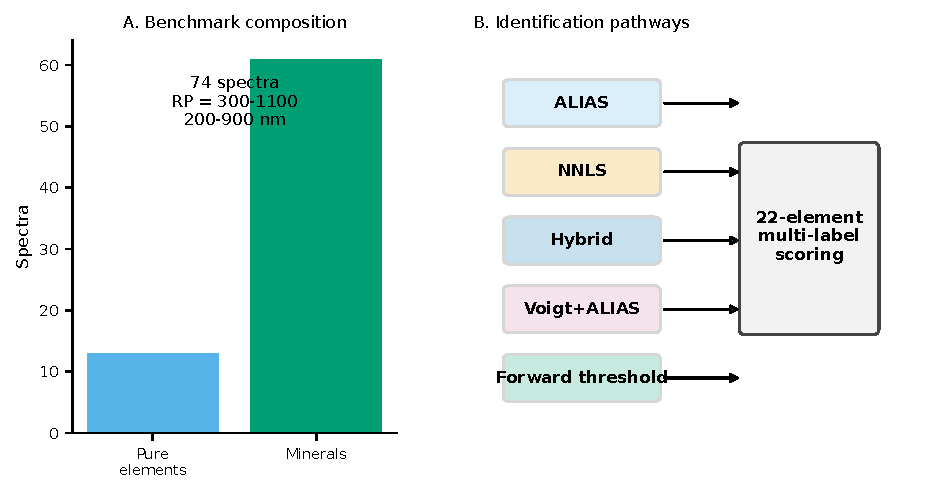
\includegraphics[width=0.95\linewidth]{figures/figure1_workflow.pdf}
  \caption{Benchmark design and pathway overview. The dataset combines pure-element and mineral spectra in a 22-element multi-label evaluation. Five pathways are compared under a common scoring protocol.}
  \label{fig:workflow}
\end{figure}

\subsection{Shared basis library}

The NNLS, hybrid, and forward-threshold pathways use a shared synthetic basis library. For each element and grid point, ionization balance is approximated with the Saha equation, excited-state populations are computed from Boltzmann factors, and line intensities are assembled from transition probabilities, statistical weights, and upper-level energies. Atomic line data are taken from the NIST Atomic Spectra Database \citep{KramidaNISTASD}. Each spectrum is convolved with a Gaussian instrumental profile and area-normalized before fitting. The basis spans 200--900 nm with 4096 wavelength pixels, a nominal FWHM of 0.5 nm, temperatures from 4000 to 12000 K in 30 steps, electron densities from $10^{15}$ to $5\times10^{17}$ cm$^{-3}$ in 10 logarithmic steps, and neutral plus singly ionized stages for 76 elements.

\begin{table}[t]
\centering
\caption{Basis-library and evaluation settings used for pathways that require synthetic spectra.}
\label{tab:basis}
\begin{tabular}{ll}
\toprule
Parameter & Value \\
\midrule
Wavelength range & 200--900 nm \\
Wavelength pixels & 4096 \\
Nominal instrument FWHM & 0.5 nm \\
Temperature grid & 4000--12000 K, 30 steps \\
Electron density grid & $10^{15}$--$5\times10^{17}$ cm$^{-3}$, 10 steps \\
Ionization stages & I and II \\
Basis elements & 76 \\
Scored elements & 22 \\
Primary metrics & Precision, recall, F$_1$, FPR, exact match \\
\bottomrule
\end{tabular}
\end{table}

The basis is intentionally simple enough to provide an interpretable physical prior, but it should not be confused with a complete plasma model. The library assumes local thermodynamic equilibrium, even though the McWhirter criterion is only a necessary condition and can be marginal for some transitions at the low-density edge of the grid \citep{Cristoforetti2010}. Only neutral and singly ionized stages are included. The 0.5 nm FWHM is reasonable near resolving powers of 600--1000, but it may mismatch spectra near the low end of the benchmark. Area normalization improves robustness to absolute intensity variation but converts NNLS coefficients into spectral-shape weights, not calibrated elemental concentrations. The temperature and density grid is evaluated only as a benchmark configuration for these spectra. Transfer to a picosecond, 1040 nm LIBS instrument should not reuse the same operating assumptions without re-estimating the plasma-parameter range, continuum behavior, gate timing, and detection thresholds for that pulse duration and optical train.

\subsection{Identification pathways}

The ALIAS pathway detects spectral peaks, applies wavelength-shift and resolving-power calibration, compares observed features with theoretical line positions, and scores candidate elements using a confidence measure based on match quality and chance-coincidence control. Detection threshold, intensity threshold factor, and chance-window scale were swept over the operating points recorded in the repository benchmark report. ALIAS represents the peak-evidence baseline: it is interpretable and fast, but exposed to chance coincidences when many database lines occupy each resolution element.

The NNLS pathway fits the observed spectrum as
\begin{equation}
I_{\mathrm{obs}}(\lambda) \approx \sum_i c_i B_i(\lambda;T,n_e) + P(\lambda),
\end{equation}
where $B_i$ is an area-normalized element basis spectrum, $c_i\ge 0$ is an NNLS coefficient, and $P(\lambda)$ is a low-order polynomial continuum. Non-negative least squares follows the classical constrained least-squares formulation of \citet{LawsonHanson1974}. An element is detected when its coefficient signal-to-noise ratio exceeds a threshold. This pathway uses global spectral context and can assign blended emission to physically plausible basis components, but it can also spread signal across many line-rich elements.

The hybrid pathway combines these two evidence streams. In the screening stage, NNLS is run with a lenient threshold to produce a candidate set. In the confirmation stage, ALIAS is restricted to those candidates and tests whether each candidate has line-level support. In intersection mode, an element must pass both stages; in union mode, it may pass either. The intersection mode is expected to improve precision by suppressing weak NNLS coefficients that have no confirmatory peak evidence, whereas union mode is expected to maximize recall at the expense of false positives.

The Voigt+ALIAS pathway applies baseline correction, peak detection, local grouping, and multi-peak Voigt fitting before running ALIAS on the reconstructed spectrum. The motivation is that deconvolution may separate blended lines before peak matching. The numerical implementation relies on nonlinear least-squares fits to grouped features and the standard complex-error-function representation of Voigt profiles \citep{Weideman1994}. The forward-threshold pathway uses the same NNLS fit as the spectral decomposition method but normalizes coefficients and detects elements whose fractional weight exceeds a threshold.

\subsection{Scoring and validity assessment}

Each pathway outputs a binary set of detected elements for each spectrum. True positives, false positives, false negatives, and true negatives are accumulated over all spectra and all 22 scored elements. The primary aggregate metrics are micro-averaged precision, recall, F$_1$, false-positive rate, and exact-match count. Exact match requires the detected element set to equal the reference set exactly for a spectrum.

The present analysis is a benchmark of fixed operating points rather than a fully confirmatory statistical trial. It reports point estimates on a small dataset, and no confidence intervals are claimed for the primary table. This choice is adequate for identifying dominant failure modes and selecting promising pathways, but a final journal submission should include grouped resampling or external validation. The strongest design for follow-up would select hyperparameters inside an inner grouped cross-validation loop, evaluate them on held-out specimens or mineral species, and report bootstrap confidence intervals for aggregate and per-element metrics. The current manuscript is written to make these limits explicit instead of treating the benchmark as a finished performance guarantee. The evaluation is also unblinded with respect to algorithm development: the benchmark report and manuscript were produced after method exploration, so the reported numbers should be treated as method-comparison evidence rather than locked, prospective validation.

\section{Results}

\subsection{Overall pathway comparison}

The hybrid NNLS+ALIAS pathway in intersection mode achieved the strongest aggregate performance among the evaluated pathways. Its best operating point, NNLS SNR threshold 1.5 and ALIAS detection threshold 0.05, gave precision 0.604, recall 0.713, F$_1$ 0.654, false-positive rate 0.053, and 16 exact matches out of 74 spectra. ALIAS alone reached F$_1$ 0.560, while Voigt+ALIAS reached 0.547. The forward-threshold method recovered more true elements than ALIAS but admitted more false positives, giving F$_1$ 0.505. Full-spectrum NNLS had the highest recall, 0.940, but its precision of 0.293 was too low for use as an element list in CF-LIBS without a subsequent confirmation stage.

\begin{table}[t]
\centering
\caption{Best observed operating point for each pathway on the 74-spectrum benchmark.}
\label{tab:overall}
\resizebox{\linewidth}{!}{%
\begin{tabular}{lllllll}
\toprule
Pathway & Configuration & P & R & F$_1$ & FPR & Exact \\
\midrule
Hybrid, intersect & nsnr=1.5, adt=0.05 & 0.604 & 0.713 & 0.654 & 0.053 & 16/74 \\
ALIAS & dt=0.05, itf=3.0 & 0.505 & 0.629 & 0.560 & 0.070 & 11/74 \\
Voigt+ALIAS & dt=0.03 & 0.488 & 0.623 & 0.547 & 0.075 & 8/74 \\
Forward threshold & ct=0.05 & 0.369 & 0.796 & 0.505 & 0.148 & 0/74 \\
Spectral NNLS & snr=3.0, T=10000 K & 0.293 & 0.940 & 0.447 & 0.236 & 2/74 \\
\bottomrule
\end{tabular}
}
\end{table}

\begin{figure}[t]
  \centering
  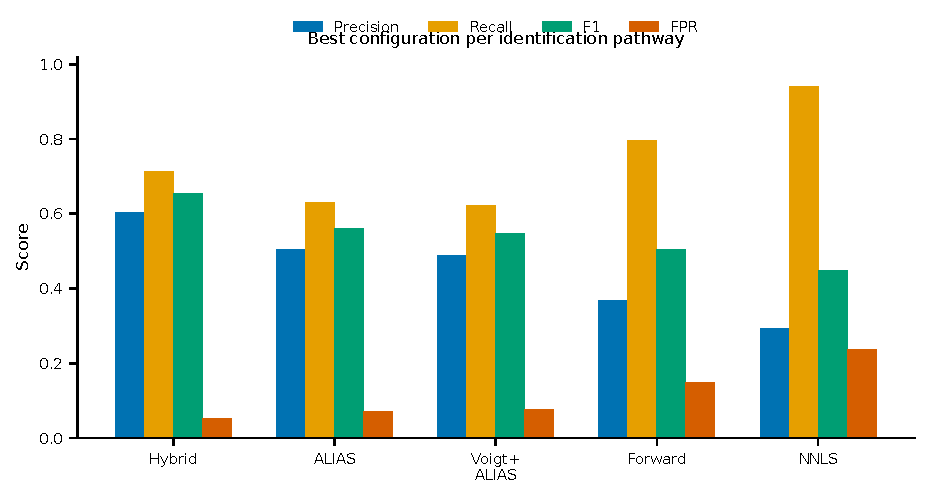
\includegraphics[width=0.95\linewidth]{figures/figure2_pathway_performance.pdf}
  \caption{Best operating points for the five tested pathways. NNLS maximizes recall but produces too many false positives. The hybrid intersection provides the best F$_1$ and the lowest false-positive rate among the evaluated methods.}
  \label{fig:pathway-bars}
\end{figure}

The pathway comparison shows that neither of the two intuitive single-method extremes is sufficient. Peak matching is conservative enough to avoid the worst NNLS false-positive burden, but it misses many formula-listed elements in blended spectra. NNLS, by contrast, recognizes much of the true spectral content but assigns small positive weights broadly across the element library. The hybrid improves performance because the two errors are not identical. Requiring both global spectral support and peak-level evidence suppresses many weak NNLS detections while retaining more true positives than ALIAS alone.

\subsection{Hybrid operating modes}

The hybrid sweep reveals a clear precision--recall separation between intersection and union logic. With the same NNLS SNR threshold of 1.5 and ALIAS detection threshold of 0.05, intersection mode gave precision 0.604 and recall 0.713, while union mode gave precision 0.308 and recall 0.952. Union mode is attractive if the only objective is to avoid missing true elements, but it is poorly matched to CF-LIBS quantification because false-positive elements enter the closure problem and can contaminate the inferred composition. Intersection mode is therefore the more defensible default for a physics-based quantitative pipeline.

\begin{figure}[t]
  \centering
  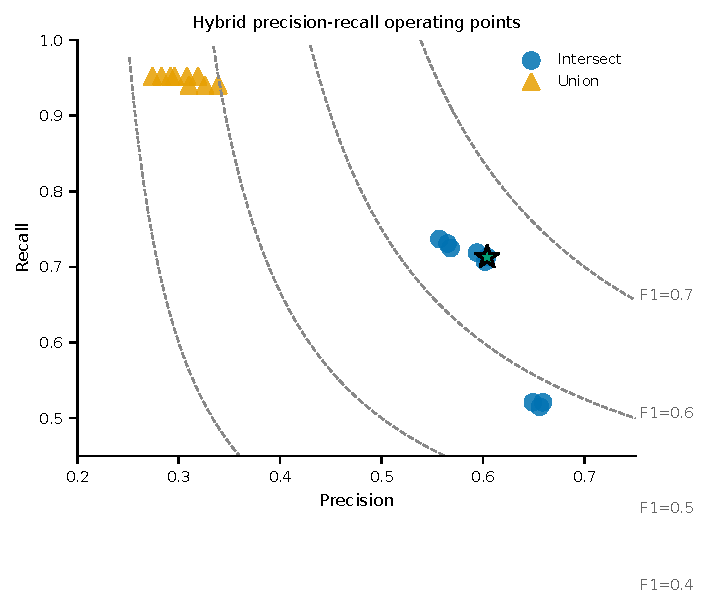
\includegraphics[width=0.70\linewidth]{figures/figure3_precision_recall.pdf}
  \caption{Precision--recall behavior for the 18 hybrid configurations. Intersection-mode configurations occupy the higher-precision region, while union-mode configurations occupy the high-recall, high-false-positive region. The star marks the best F$_1$ operating point.}
  \label{fig:pr}
\end{figure}

\subsection{Per-element behavior}

The aggregate metrics hide substantial element-specific structure. The hybrid method reached precision 1.00 for Si, Al, Fe, Li, Co, and Ni. For Si and Al, the hybrid also retained high recall, 0.95 and 0.90, respectively. These elements are important because they represent major rock-forming constituents and are common targets in geological LIBS workflows. Fe had perfect precision but low recall, 0.44, indicating that the hybrid is cautious when Fe emission is blended or weak. Mg, Ca, K, Ti, and Pb showed mixed precision--recall trade-offs. Zn and Zr were not recovered under the evaluated conditions.

\begin{figure}[t]
  \centering
  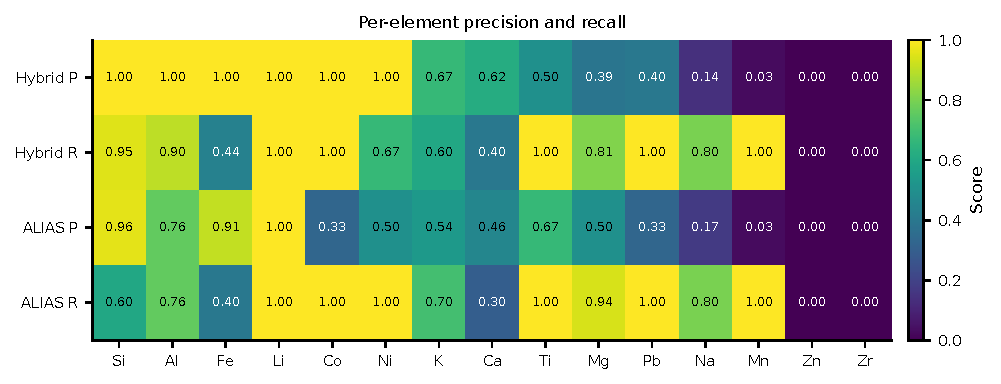
\includegraphics[width=0.95\linewidth]{figures/figure4_per_element.pdf}
  \caption{Per-element precision and recall for the best hybrid and ALIAS operating points. Hybrid performance is strong for several major rock-forming and metallic elements, but Mn and Na remain low-precision detections.}
  \label{fig:per-element}
\end{figure}

Mn and Na dominate the false-positive structure. Mn is line-rich across the visible and near-UV regions, so at low resolving power it can match many unrelated blend envelopes by chance. Na is different: its D-line emission near 589 nm is intense and susceptible to contamination, and its sparse practical evidence set makes line confirmation fragile. Both elements can therefore pass peak-level and full-spectrum gates even when their formula-based label is absent. These errors should not be interpreted solely as algorithmic defects; in the absence of specimen-specific assays, some apparent false positives may reflect real impurities or contamination. Nevertheless, the consistency of the pattern indicates that Mn and Na need special, resolving-power-aware treatment in blind low-resolution searches.

\subsection{Wavelength-shift stress behavior}

Repository validation also includes a synthetic wavelength-shift stress test for representative identifier variants. Under imposed shifts of -1, 0, and +1 nm, ALIAS F$_1$ varied from 0.273 to 0.529, the comb-style method varied from 0.160 to 0.467, and a correlation method varied from 0.229 to 0.333. The test is not the same as the Aalto mineral benchmark and should not be mixed directly with the primary performance table, but it reinforces a practical point: low-resolution element identification is sensitive to wavelength calibration. For any deployable CF-LIBS pipeline, wavelength-axis correction and calibration diagnostics should be treated as first-order components rather than preprocessing details.

\begin{figure}[t]
  \centering
  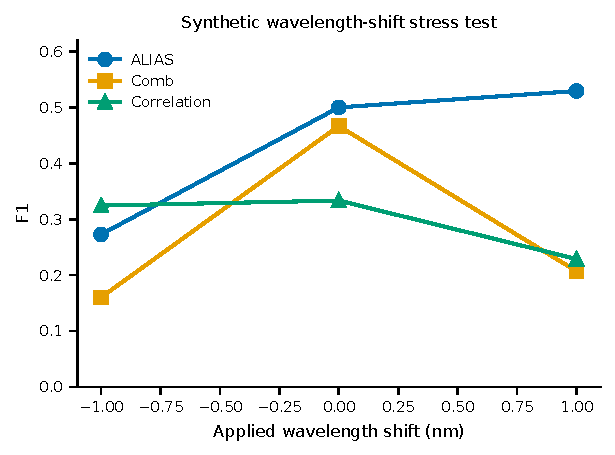
\includegraphics[width=0.70\linewidth]{figures/figure5_shift_stress.pdf}
  \caption{Synthetic wavelength-shift stress test from repository validation. The result is separate from the Aalto benchmark but shows that nanometer-scale calibration shifts can substantially change identification performance.}
  \label{fig:stress}
\end{figure}

\section{Discussion}

The central result is that a two-stage architecture outperforms either peak matching or full-spectrum fitting alone in this low-resolution setting. This outcome is physically plausible. NNLS uses the full spectral shape, so it can extract information from blended emission that would be difficult to interpret as isolated lines. However, its non-negativity constraint does not prevent many line-rich species from receiving weak positive coefficients. ALIAS uses discrete line evidence and chance-coincidence control, so it suppresses some spurious coefficients, but it is vulnerable when blend envelopes replace isolated peaks. The hybrid gains because each stage rejects a different subset of errors.

The magnitude of improvement is meaningful but bounded. The best hybrid F$_1$ of 0.654 is a useful baseline, not a complete solution. A false-positive rate of 0.053 over 22 elements and 74 spectra still produces enough incorrect elements to matter in downstream quantification. Exact identification occurred in only 16 spectra. In practical CF-LIBS, an exact element list is often more important than aggregate F$_1$ because the closure equation couples all included species. A method that improves average precision while still inserting Mn or Na into many spectra can still degrade quantitative results.

The benchmark also clarifies why Voigt deconvolution did not rescue peak matching. Deconvolution is attractive when spectra contain moderately overlapping peaks and the number of components in each group is small. At resolving powers below 1000 across a transition-dense LIBS band, many features are not simple two- or three-line overlaps but compound envelopes with many possible contributors. The inverse problem becomes underdetermined, and nonlinear fitting can create plausible peak shapes that do not correspond to uniquely assignable transitions. In this regime, deconvolution can add computational cost without adding reliable information.

The strongest scientific risk in the present study is construct validity of the labels. Formula-derived mineral labels are useful for benchmarking, but they are not specimen-specific truth. A natural mineral spectrum can legitimately contain Na, Mn, Fe, or other elements omitted from a nominal formula. The benchmark therefore measures agreement with a practical reference convention, not absolute chemical truth. This issue is especially important for the two most problematic elements. Some Na detections may be real contamination, and some Mn detections may reflect trace impurities. Future work should pair low-resolution spectra with independent compositional assays such as XRF, ICP-MS, or electron microprobe measurements, and should record replicate spectra so that shot-to-shot stability can be separated from label uncertainty.

Internal validity is also limited by the use of point estimates from a small benchmark. The operating points were selected from finite parameter sweeps and evaluated on the same corpus. That is acceptable for exploratory method comparison, but it can overstate performance if reported as final generalization accuracy. A submission-ready confirmatory study should use grouped cross-validation or an external test set, report uncertainty intervals, and stratify results by sample class, resolving power, label cardinality, and element support. Rare elements require particular caution because a single false positive or false negative can dominate per-element precision or recall.

The implications for CF-LIBS pipeline design are nevertheless clear. Low-resolution blind identification should avoid single-evidence decisions. A reasonable conservative workflow is to use full-spectrum fitting to generate candidates, require independent line-level confirmation, and then apply resolving-power-aware rules for known pathological elements. For Mn and Na at resolving powers below 1000, the pipeline should either mark detections as low-confidence, require additional corroborating lines or replicate persistence, or defer the decision to a higher-resolution measurement. Where quantitative CF-LIBS is the end goal, the element list should be iteratively checked against residual structure and physically plausible concentrations rather than accepted as a one-shot output.

The work also suggests several productive extensions. First, the synthetic basis should be matched to each spectrum's effective resolution rather than using a single 0.5 nm FWHM. Second, temperature and electron density should be inferred jointly or marginalized instead of using fallback values in the NNLS stage. Third, the hybrid decision rule could be replaced by calibrated probabilistic fusion of NNLS coefficients, ALIAS scores, calibration residuals, and replicate consistency. Fourth, a resolving-power series should be constructed by degrading high-resolution spectra or comparing against instruments such as ChemCam and SuperCam so that the transition from blend-envelope matching to line-resolved matching can be measured directly.

\section{Conclusions}

This benchmark shows that low-resolution blind element identification for CF-LIBS benefits from combining global physical fitting with peak-level confirmation. On 74 mineral and pure-element spectra at resolving powers of approximately 300--1100, a hybrid NNLS+ALIAS intersection method achieved the best aggregate performance among the evaluated pathways, with precision 0.604, recall 0.713, F$_1$ 0.654, false-positive rate 0.053, and 16 exact matches. Full-spectrum NNLS alone recovered most true elements but produced too many false positives, while ALIAS alone was more conservative but less complete. The hybrid result is therefore the strongest current baseline in this codebase for low-resolution element identification, but it remains an exploratory benchmark result rather than an externally validated deployment claim.

The study also demonstrates that the problem remains open. Mn and Na are persistent false-positive sources, formula-derived mineral labels limit construct validity, and point-estimate benchmarking cannot replace independent chemical validation. A journal-ready experimental extension should add specimen-specific assays, grouped uncertainty estimates, replicate stability tests, and a resolving-power dependence study. Within those limits, the present article provides a defensible framework for evaluating CF-LIBS element-identification pathways and a practical target for future algorithmic and instrumental improvements.

\section*{Data and Code Availability}

The manuscript, figure-generation script, benchmark report, and validation artifacts are maintained in the CF-LIBS-improved repository. The primary benchmark values used here are traceable to the element-identification benchmark report and the calibration-stress validation artifact in the repository. The manuscript figures can be regenerated with the Python script stored alongside this manuscript.

\section*{Conflict of Interest}

The author declares no competing financial interests. Funding and affiliation statements should be completed before journal submission.

\bibliography{refs}

\end{document}
